\section{Simulator}


\subsection{Scene simulation}

We use Unity3D to simulate scene like a truth supermarket, it is length and width and height of the scene are 40m, 25m, 6m, and aisle width is 2.7m.
Bin width is 2.35m and height is 1.7m.
Then we put the cameras on the shelves, the height is 2.22m, set cameras 6.8m apart from the previous calculations, and the h-fov is 1.2 bin.
A four-direction camera is placed every three meters above the corridor, the 4 cameras are 4 directions, and height of them are 3.5m.
Our scene is shown in the figure.6.
\begin{figure}[htbp]
\centerline{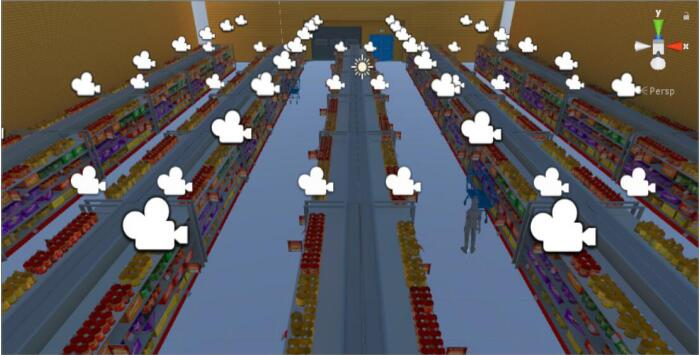
\includegraphics[width=8.2cm,scale=0.9]{supermarket.jpg}}
\caption{Page Size and Optical Resolution}
\label{fig}
\end{figure}

We set the h-fov is 1.2 bin, which let camera can cover 2 bin, in order to get a clearer picture. In figure.7, we can see the cameras which on shelves can clearly obtain the type and quantity of goods, this provides a great help for our later identification.
\begin{figure}[htbp]
\centerline{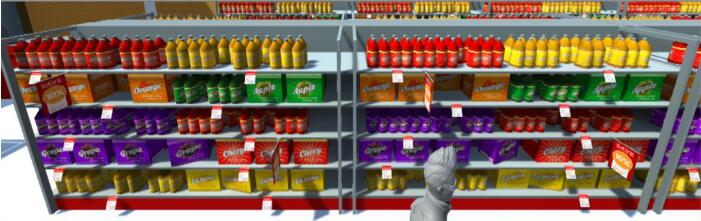
\includegraphics[width=7cm,scale=0.8]{shelves.jpg}}
\caption{Page Size and Optical Resolution}
\label{fig}
\end{figure}

\subsection{Item Recognition}
In this section, we will introduce this system Item Recognition. In Unity3D we can use the clear screenshot F9 to get the picture which is describe the items type and quantity on shelves, and it is resolution is 1600*1200.

We use the sample picture to verify the Item Recognition. There is a picture about Yakult which we get in web, and then we put it in the identity system what we build based on YOLOv3\cite{yolov3}. As for figure.8, we can accurately identity the types of articles and number of articles, it uses boxes to present items tested.
\begin{figure}[htbp]
\centerline{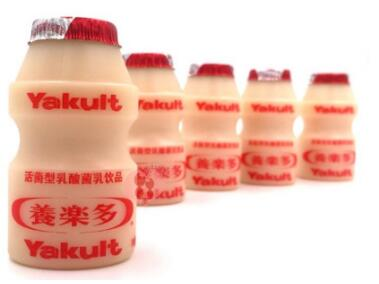
\includegraphics[width=3.5cm,scale=0.6]{Yakult.jpg} 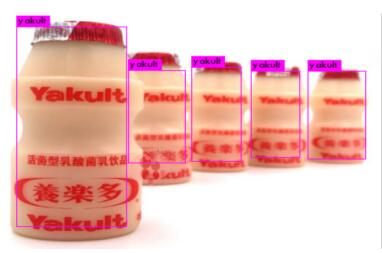
\includegraphics[width=3.5cm,scale=0.6]{Yakult_new.jpg}}
\caption{.}
\label{fig}
\end{figure}

Their recognition rates ranged from left to right is 100\%, 86\%, 100, 100, 100. Then we use the other pictures to do Item Recognition test, we can still get high recognition rate and accurately obtain the type and quantity of goods. Thus it can be seen, our experiment is feasibility and accuracy.
